\documentclass[a4paper, twoside]{report}
\setcounter{tocdepth}{3}
\setcounter{secnumdepth}{3}
%Language and font encodings
\usepackage[english]{babel}
\usepackage[utf8]{inputenc}

\usepackage{titlesec}
\titleformat{\chapter}[display]
  {\Huge\bfseries}
  {}
  {0pt}
  {\thechapter.\ }

\titleformat{name=\chapter,numberless}[display]
  {\Huge\bfseries}
  {}
  {0pt}
  {}

%Sets page size and margins
\usepackage[a4paper,top=3cm,bottom=2cm,left=3cm,right=3cm,marginparwidth=1.75cm]{geometry}

%Useful packages
\usepackage{array}
\usepackage{amsmath}
\usepackage{amssymb}
\usepackage{url}
\usepackage{listings}
\usepackage{color}
\usepackage{longtable}
\usepackage{graphicx}
\usepackage{pdfpages}
\usepackage{enumitem}
\usepackage[hidelinks]{hyperref}
\usepackage{siunitx}
\usepackage{pdfpages}

\title{A Visual GUI Tool for Replacing Post-it Note in Image, Video and Live Stream with Customized Image}

\begin{document}
\begin{titlepage}

\newcommand{\HRule}{\rule{\linewidth}{0.3mm}} % Defines a new command for the horizontal lines, change thickness here


\center % Center everything on the page

\includegraphics[width=9cm]{title/logo.png}\\[1.5cm]

%	TITLE SECTION

\makeatletter
\HRule \\[0.8cm]
{ \huge \bfseries \@title}\\[0.4cm] % Title of your document
\HRule \\[0.5cm]

%	HEADING SECTIONS

\textsc{\Large Ravensburg-Weingarten University}\\[0.3cm] 
\textsc{\large Electrical Engineering and Information Technology}\\ [1.5cm]


\large Bachelor Project Report  \large\\
\textbf{Period:} 01.07.2020 - 30.09.2020\large\


%	AUTHOR SECTION

\vspace{2.5cm}

\begin{minipage}{0.4\textwidth}
\begin{flushleft} \large
\emph{Supervisor:} \\ Prof. Dr. Markus \textsc{Pfeil} 
\end{flushleft}
\end{minipage}
~
\begin{minipage}{0.4\textwidth}
\begin{flushright}\large
\emph{Author:}\\ Siyi \textsc{Dai} \\
\emph{Matrikel-Nr.:}\\ 29245 \\

\end{flushright}
\end{minipage}\\[2cm]

\makeatother
%	DATE SECTION

{\large \today}\\[7cm] 



\vfill % Fill the rest of the page with whitespace

\end{titlepage}




\newpage
\tableofcontents
\newpage

\chapter{Introduction}
\section{Definition of Tasks}
\noindent The project tasks are focused on developing graphical user interfaces (GUI) for replacing the post-it note area in image, video and live stream with loaded image using OpenCV-Python library.  \\ \par

\noindent GUI is a form of user interface that allows users to interact with electronic devices through graphical icons, instead of text-based user interfaces, typed command labels or text navigation.  \\ \par

\noindent OpenCV-Python is a library of Python bindings designed to solve computer vision problems. As an interdisciplinary scientific field, computer vision deals with how computers can gain high-level understanding from digital images or videos.    \\ \par

\chapter{Environment Specification}
\noindent The work environment is composed of two sides. The hardware environment which presents the machines or components being used while running code. The software environment which represents the advanced programming interfaces, integrated development environments, editors, technologies and tools being used.  \\ \par

\section{Hardware Environment}
\noindent The table describes the used computer for work while two BenQ Corporation 32" monitors were used. \\ \par

\begin{table}[h]
\centering
\begin{tabular}{|c|c|}
\hline
PC & HP ZBook 15 G5 (3AX13AV) \\
\hline
CPU & Intel(R) Core(TM) i7-8850H CPU @ 2.60GHz \\
\hline
RAM & 32GB \\
\hline
OS & Ubuntu 18.04.3 LTS \\
\hline
Graphics Card & NVIDIA Quadro P1000 Mobile\\
\hline
\end{tabular}
\caption{Characteristics of used computer}
\end{table}


\section{Software Environment}
\paragraph{Python 3.6.10 :: Anaconda, Inc.}
\textit{Python} is an interpreted, high-level, general-purpose programming language. The internship tasks are all coded in \textit{Python 3.6.10} within help of \textit{Anaconda}, which is a \textit{Python} and \textit{R} distribution including the core python language, 100+ Python libraries and package manager \textit{conda}. \\ \par

\paragraph{Visual Studio Code}
\textit{Visual Studio Code} is a free source-code editor  made by \textit{Microsoft} for \textit{Windows}, \textit{Linux}, \textit{macOS}. Features include support for debugging, syntax highlighting, intelligent code completion, snippets, code refactoring, and embedded Git.  \\ \par

\paragraph{PyQt5}
\textit{PyQt5} is a GUI develop application provided by \textit{Python}. It is cross-platform GUI toolkit, a set of python bindings for \textit{Qt v5}. An interactive desktop application can be developed with much easier because of the tools and simplicity provided by this library. \\ \par

\newpage
\noindent \textsc{Modules and Classes: } While the designation of Exporter and Visualizer, various modules and classes from \textit{PyQt5} have been used.   \\ \par
{\renewcommand{\arraystretch}{1.5}%
\begin{table}[h!]
\centering
\begin{tabular}{ m{2cm}| m{.8\textwidth}  }
Modules & Classes \\
\hline
\textit{Qt Core} &\textit{QTimer, Qt} \\
\hline
\textit{Qt gui} &\textit{QPixmap, QColor, QImage } \\
\hline
\textit{Qt Widgets} & \textit{QMainWindow, QColorDialog, QDialog} \\
\end{tabular}
\caption{Modules and Classes being used for developing UI tools}
\end{table} \quad

\paragraph{Qt Creator}
\textit{Qt Creator} includes a code editor and integrates \textit{Qt Designer} for designing and building GUIs from \textit{Qt widgets}. After layout designing and objects naming in \textit{Qt Creator}, a form implementation could be generated from reading ui file by \textit{PyQt5 UI code generator 5.9.2}. \\ \par



\paragraph{OpenCV-Python}
\textit{OpenCV-Python}is the Python API of OpenCV. \\ \par

\noindent \textsc{Functions: } While the designation of post-it replacer, various functions from \textit{cv2}, version 4.1.2, have been used.   \\ \par
{\renewcommand{\arraystretch}{1.5}%
\begin{table}[h!]
\centering
\begin{tabular}{ m{5cm}| m{.6\textwidth}  }
Functions & Usages \\
\hline
\textit{cv2.VideoCapture()} & get a video capture object for the camera or file path\\
\hline
\textit{cv2.boundingRect()} &calculates and returns the minimal up-right bounding rectangle for the specified point set or non-zero pixels of gray-scale image \\
\hline

\textit{cv2.findContours()} &retrieves contours from the binary image using the algorithm \textsc{[Suzuki85]} \\
\hline
\textit{cv2.CHAIN{\_}APPROX{\_}SIMPLE} &compresses horizontal, vertical, and diagonal segments and leaves only their end points \\
\hline
\textit{cv2.RETR{\_}TREE} &retrieves all of the contours and reconstructs a full hierarchy of nested contours \\
\hline

\textit{cv2.cvtColor()} &convert an image from one color space to another \\
\hline
\textit{cv2.COLOR{\_}RGB2BGR} &convert from RGB to BGR color spaces  \\
\hline
\textit{cv2.COLOR{\_}BGR2RGB} &convert from BGR to RGB color spaces  \\
\hline

\textit{cv2.inRange()} &Checks if array elements lie between the elements of two other arrays \\
\end{tabular}
\caption{Modules and Classes being used for developing UI tools}
\end{table} \quad

\chapter{Approach and Method}
\paragraph{Read} Whether in picture mode, video mode or camera mode, the input stream needs to be read frame by frame, which means that it is resolved to several pictures, and detecting the target object in accordance with the input color range.      \\ \par

\noindent After the picture is read, it is stored in the form of a matrix, such as a 1280x720 color picture. If read according to RGB three channels, the picture becomes a 1280x720x3 matrix, and the three values at each position are the RGB channels values.     \\ \par

\paragraph{Mask} The role of the mask is to limit the color range by setting the lower and upper limitation of RGB value. The colors between the lower and upper limits will be reserved as white, and the colors in the other ranges are all converted to black, so that a binary value with only black and white is obtained.      \\ \par

\begin{figure}[h!]
\centering
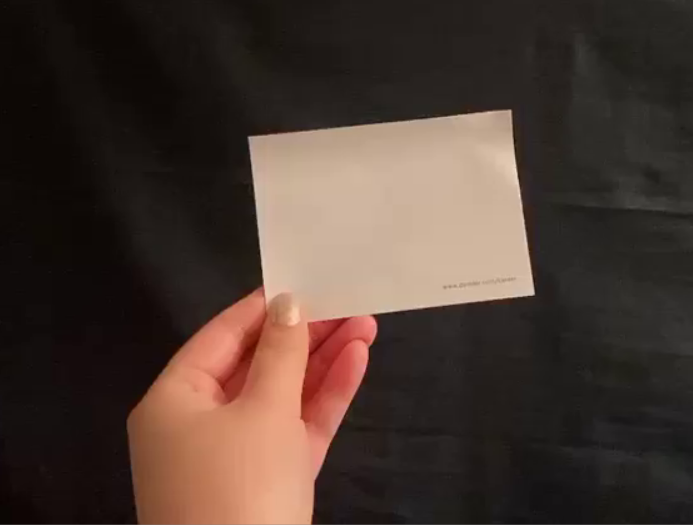
\includegraphics[width=.45\textwidth]{mask.png}
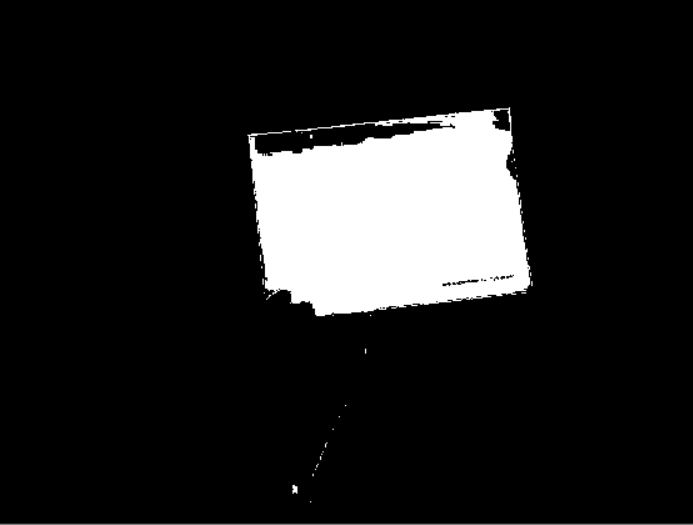
\includegraphics[width=.45\textwidth]{mask1.png}
\caption{The mask obtained with the yellow post-it note in the video and the original image}
\end{figure}

\noindent Post-it note within the color range will be retained and the other colors will be ignored. This is also the reason that the color of post-it notes and the background color are required to be as different as possible.      \\ \par


\newpage
\paragraph{Determine the Boundary} After obtaining the mask, we need to determine the boundary of the white area in the mask. This process is implemented by the function \textit{cv2.findContours()}.      \\ \par


\noindent This function will group all the continuous white pixels into one area and use the smallest rectangle bounding  box to frame these discrete areas, which creates a lot of unconnected areas in the mask. \\ \par

\begin{figure}[h!]
\centering

\includegraphics[width=.45\textwidth]{frame.png}
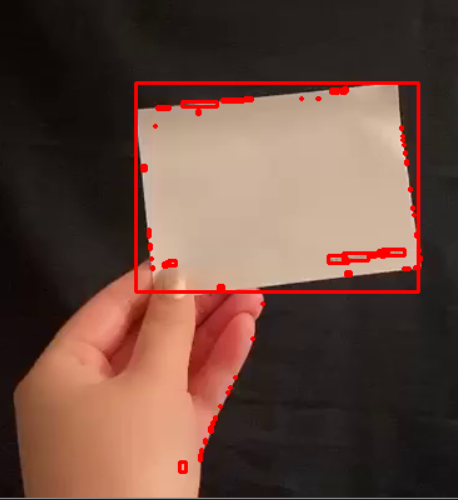
\includegraphics[width=.45\textwidth]{frame1.png}
\caption{Determine the boundary of the white area in the mask with function \textit{cv2.findContours()}}
\end{figure}


\noindent Many discrete rectangular areas will be detected. The function \textit{cv2.findContours()} will return the coordinates of the upper left corner and the lower right corner of all rectangular boxes.  \\ \par

\paragraph{Find the Biggest Bounding Box} we calculate the area of all rectangular boxes according to the width and height of the rectangular boxes, and choose the largest one. \\ \par

\begin{figure}[h!]
\centering
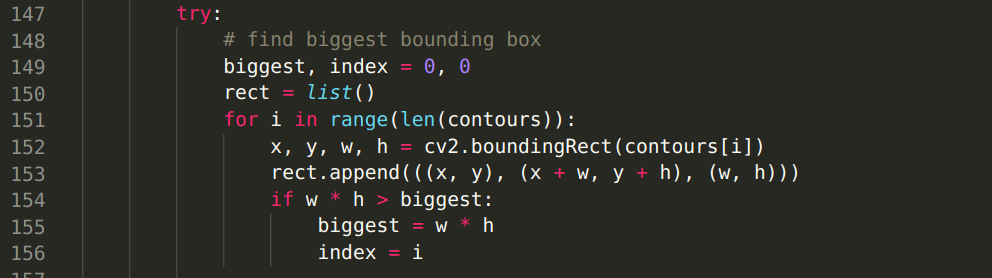
\includegraphics[width=.9\textwidth]{code.png}
\caption{The function used for finding the biggest bounding box among all white area}
\end{figure}

\newpage
\paragraph{Transform} For better visualization, the replacement area will be half-sized to the middle of the post-it, which is approached by the following function.

\begin{figure}[h!]
\centering
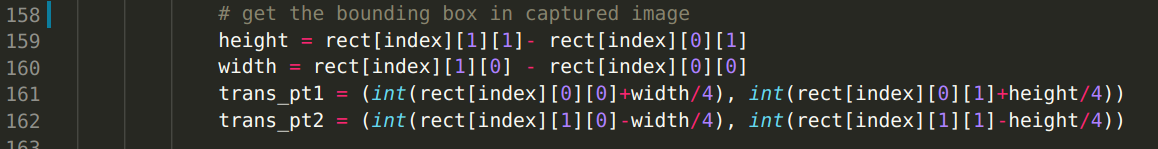
\includegraphics[width=.9\textwidth]{code1.png}
\caption{The function used for finding the half-sized bounding box in the middle of the post-it}
\end{figure}

\paragraph{Resize and Replace} After obtaining the width and height of the largest rectangular box, that is, w and h, the selected replacement image will be read in RGB format and resize it into a matrix of (w/2, h/2, 3), replacing the pixels in the largest rectangular box in the current frame. \\ \par



\noindent Since the detected rectangle is a rectangle, the picture can only be replaced in the positive direction, and the oblique post-it note will replace the smallest bounding rectangle, which is also in the positive direction.\\ \par

\begin{figure}[h!]
\centering
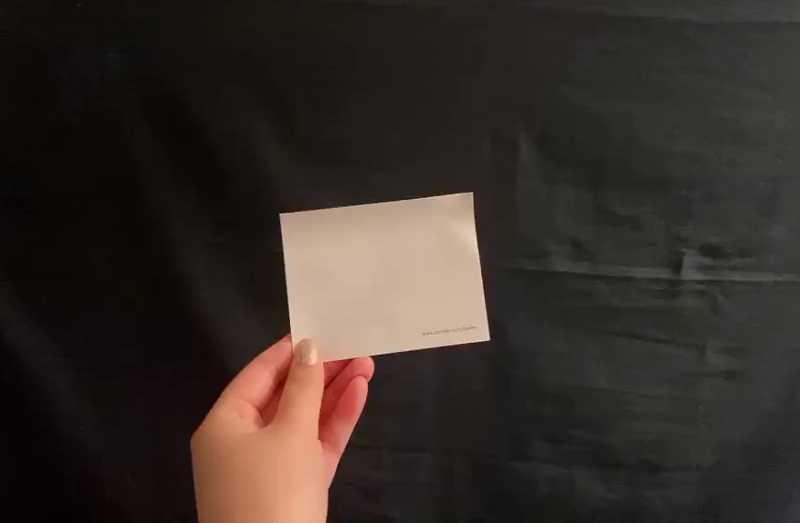
\includegraphics[width=.45\textwidth]{video.png}
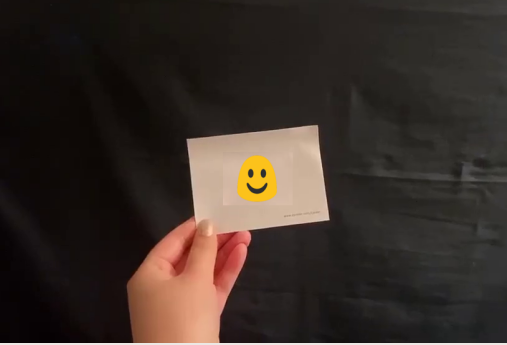
\includegraphics[width=.45\textwidth]{video1.png}
\caption{The function used for finding the half-sized bounding box in the middle of the post-it}
\end{figure}

\chapter{Post-it Replacer}
\section{Project Structure}

\noindent A graphical user interfaces (GUI) for replacing the post-it note area in image, video and live stream with loaded image using OpenCV-Python library has been successfully developed in this project.    \\ \par

\noindent The project folder is divided as:
\begin{itemize}
\item \textbf{dialogs} folder for storing IO dialog related scripts
\item \textbf{ui and ui{\_}py} folders for storing the \textit{.ui} file and the \textit{.py} file generated from reading \textit{.ui} file by \textit{PyQt5 UI code generator 5.9.2}
\item \textbf{windows} folder for storing mainwindow related script
\item \textbf{post{\_}it{\_}replace.py} executable file for starting the GUI 
\end{itemize}


\begin{figure}[h!]
\centering
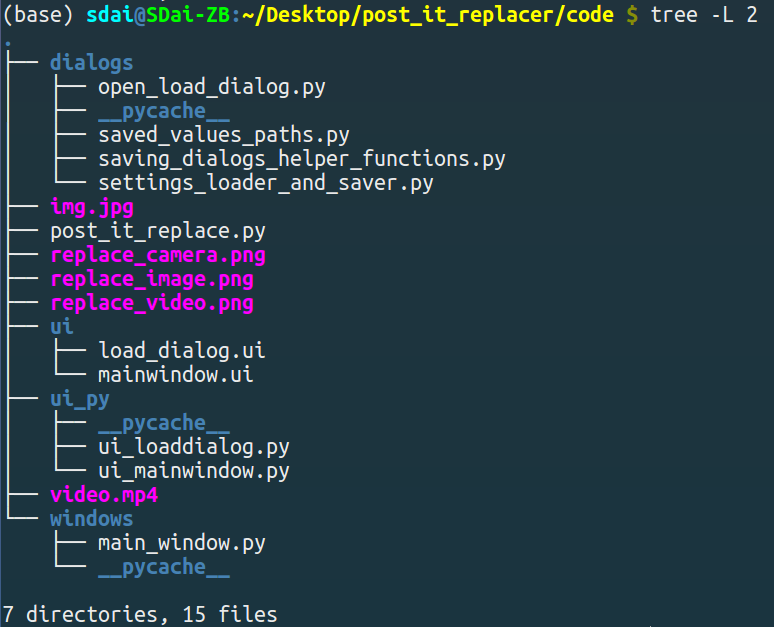
\includegraphics[width=.69\textwidth]{structure.png}
\caption{The project structure in level 2}
\end{figure}




\newpage
\section{Dialogs}
\noindent With an IO dialog, the user can conveniently select the original image or video with post-it to be replaced with as well as the replace image.   \\ \par

\begin{figure}[h!]
\centering
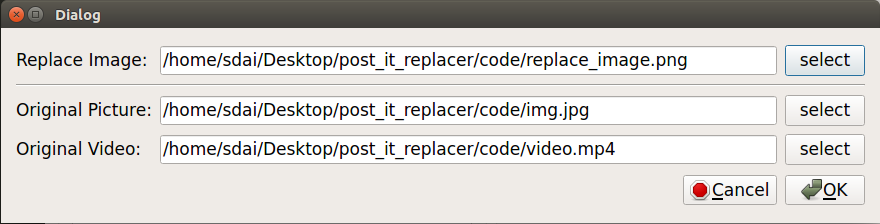
\includegraphics[width=.9\textwidth]{dialog.png}
\caption{Dialog for loading replace image, original picture and original video}
\vspace{5mm}
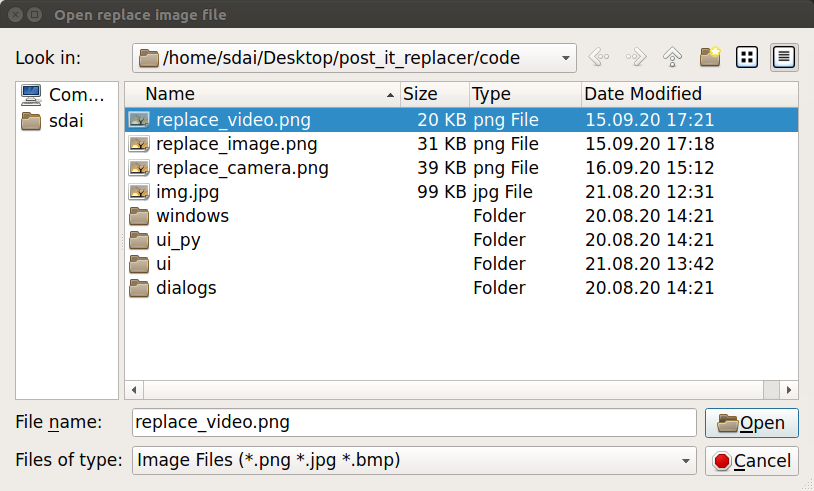
\includegraphics[width=.9\textwidth]{dialog_load.png}
\caption{Select image or video from system file path}
\end{figure}

\subsection{Code}

\begin{itemize}
\item open{\_}load{\_}dialog.py
\item saved{\_}values{\_}paths.py
\item saving{\_}dialogs{\_}helper{\_}functions.py
\item settings{\_}loader{\_}and{\_}saver.py
\item load{\_}dialog.ui
\item ui{\_}loaddialog.py
\end{itemize}

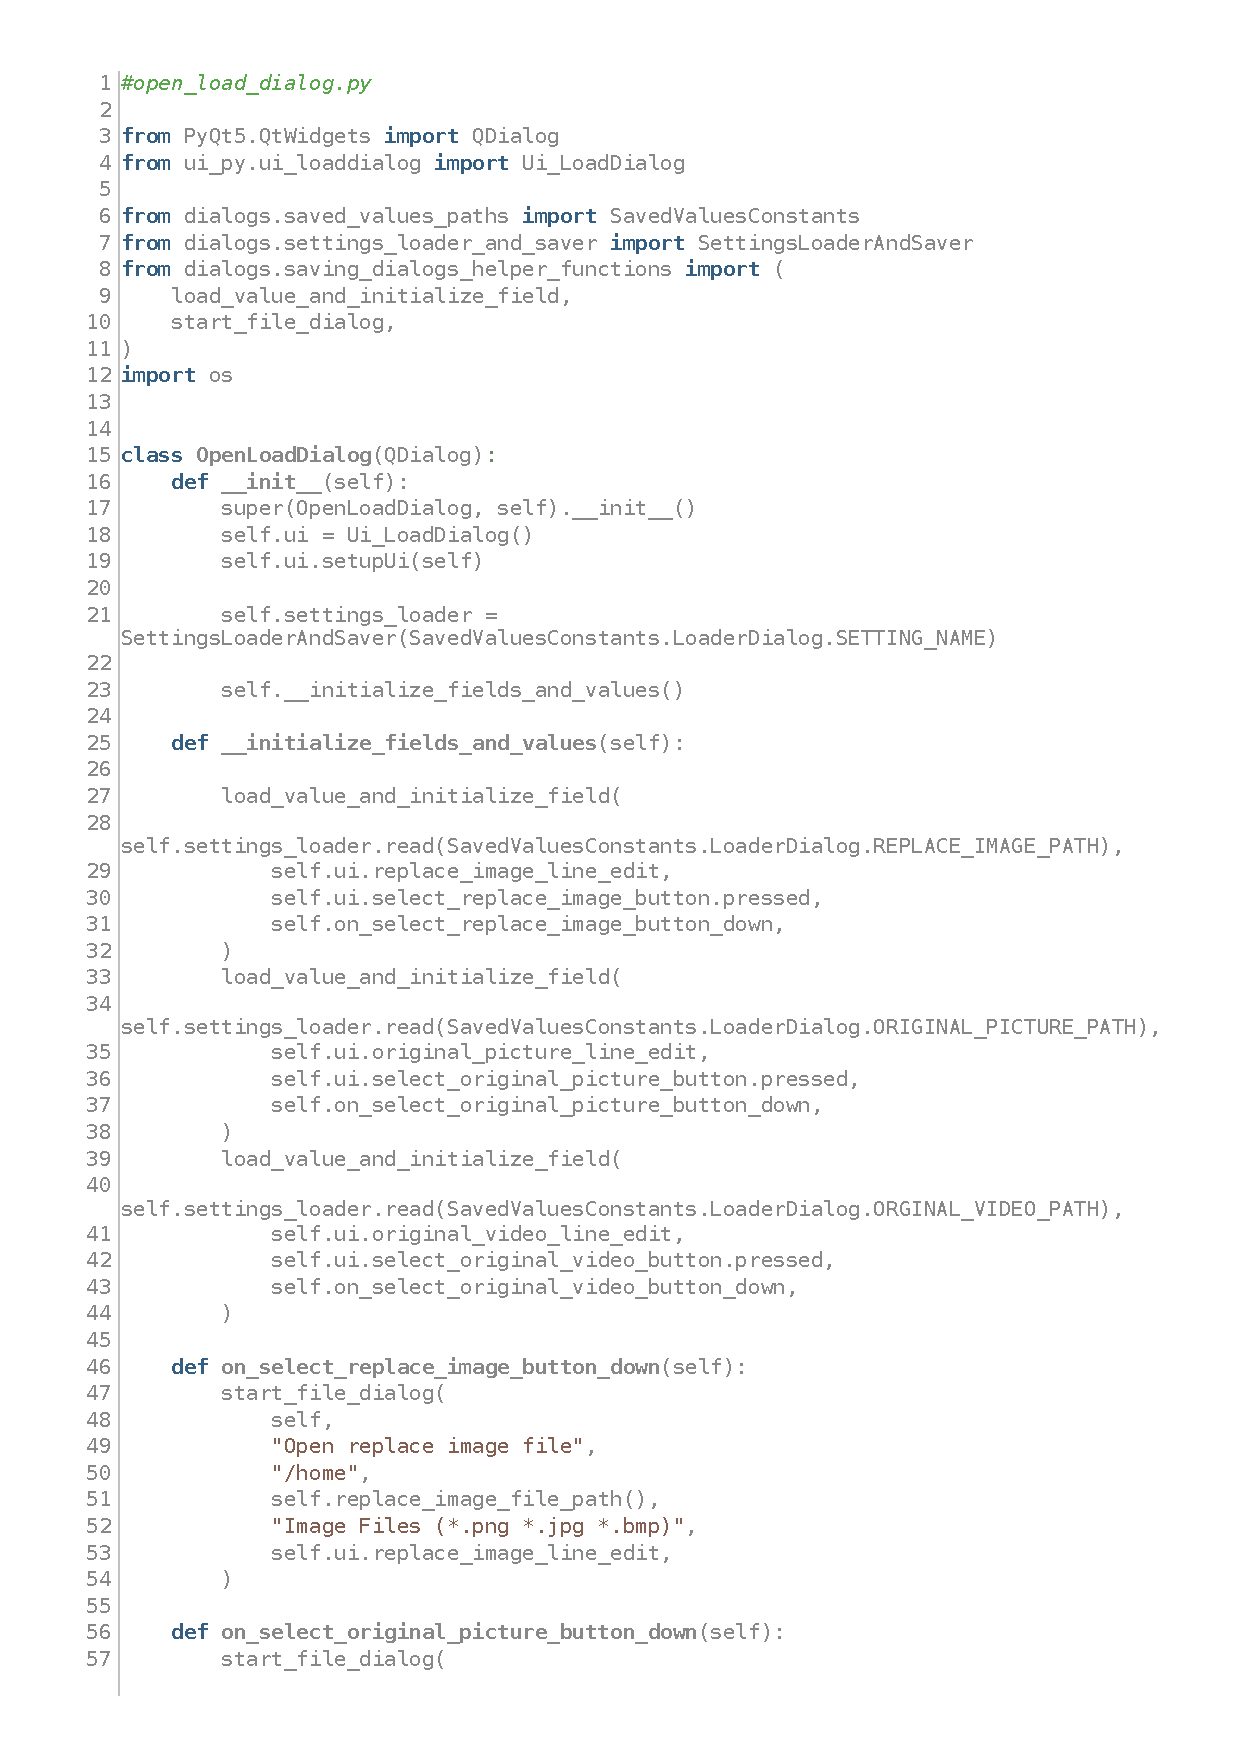
\includepdf[pages=-,pagecommand={},delta=3mm 3mm, frame = true, width=\textwidth]{open_load_dialog.pdf}
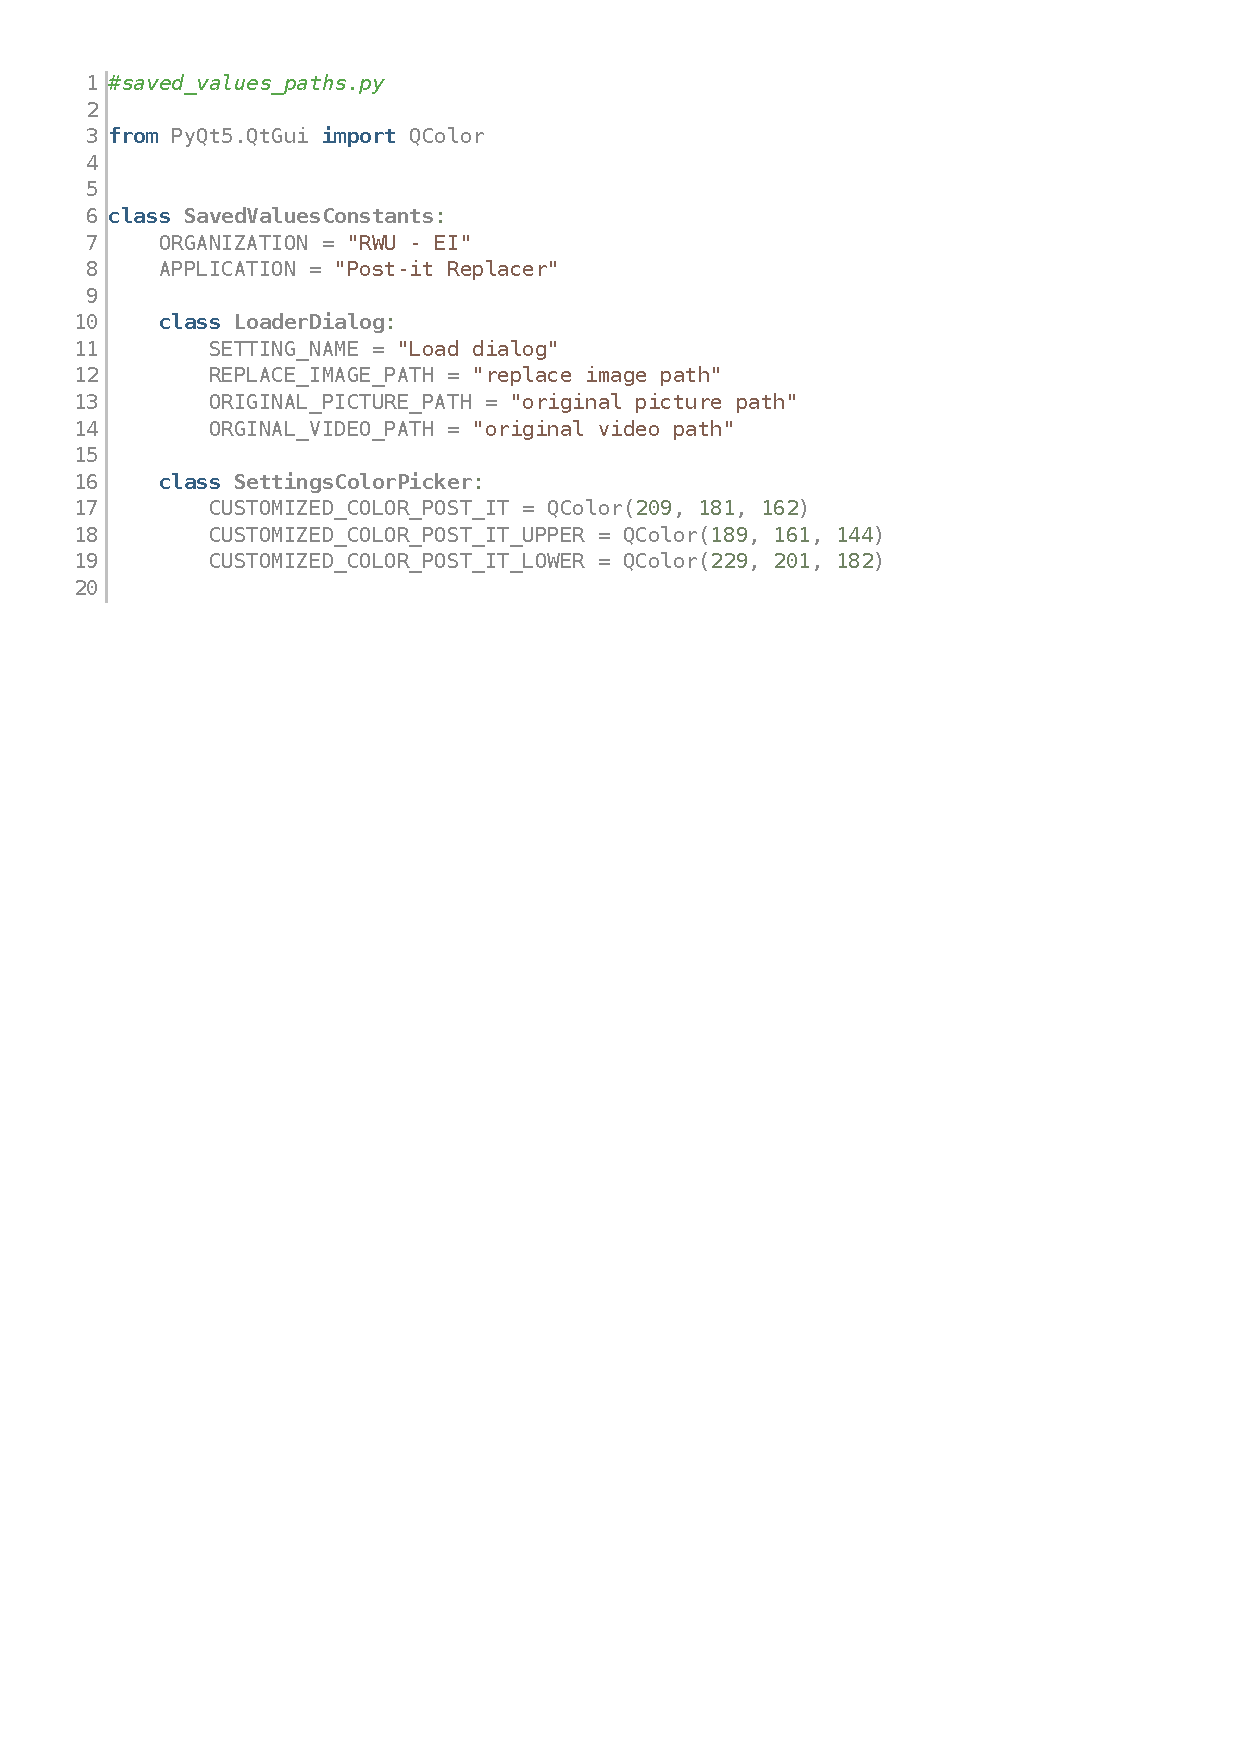
\includepdf[pages=-,pagecommand={},delta=3mm 3mm, frame = true, width=\textwidth]{saved_values_paths.pdf}
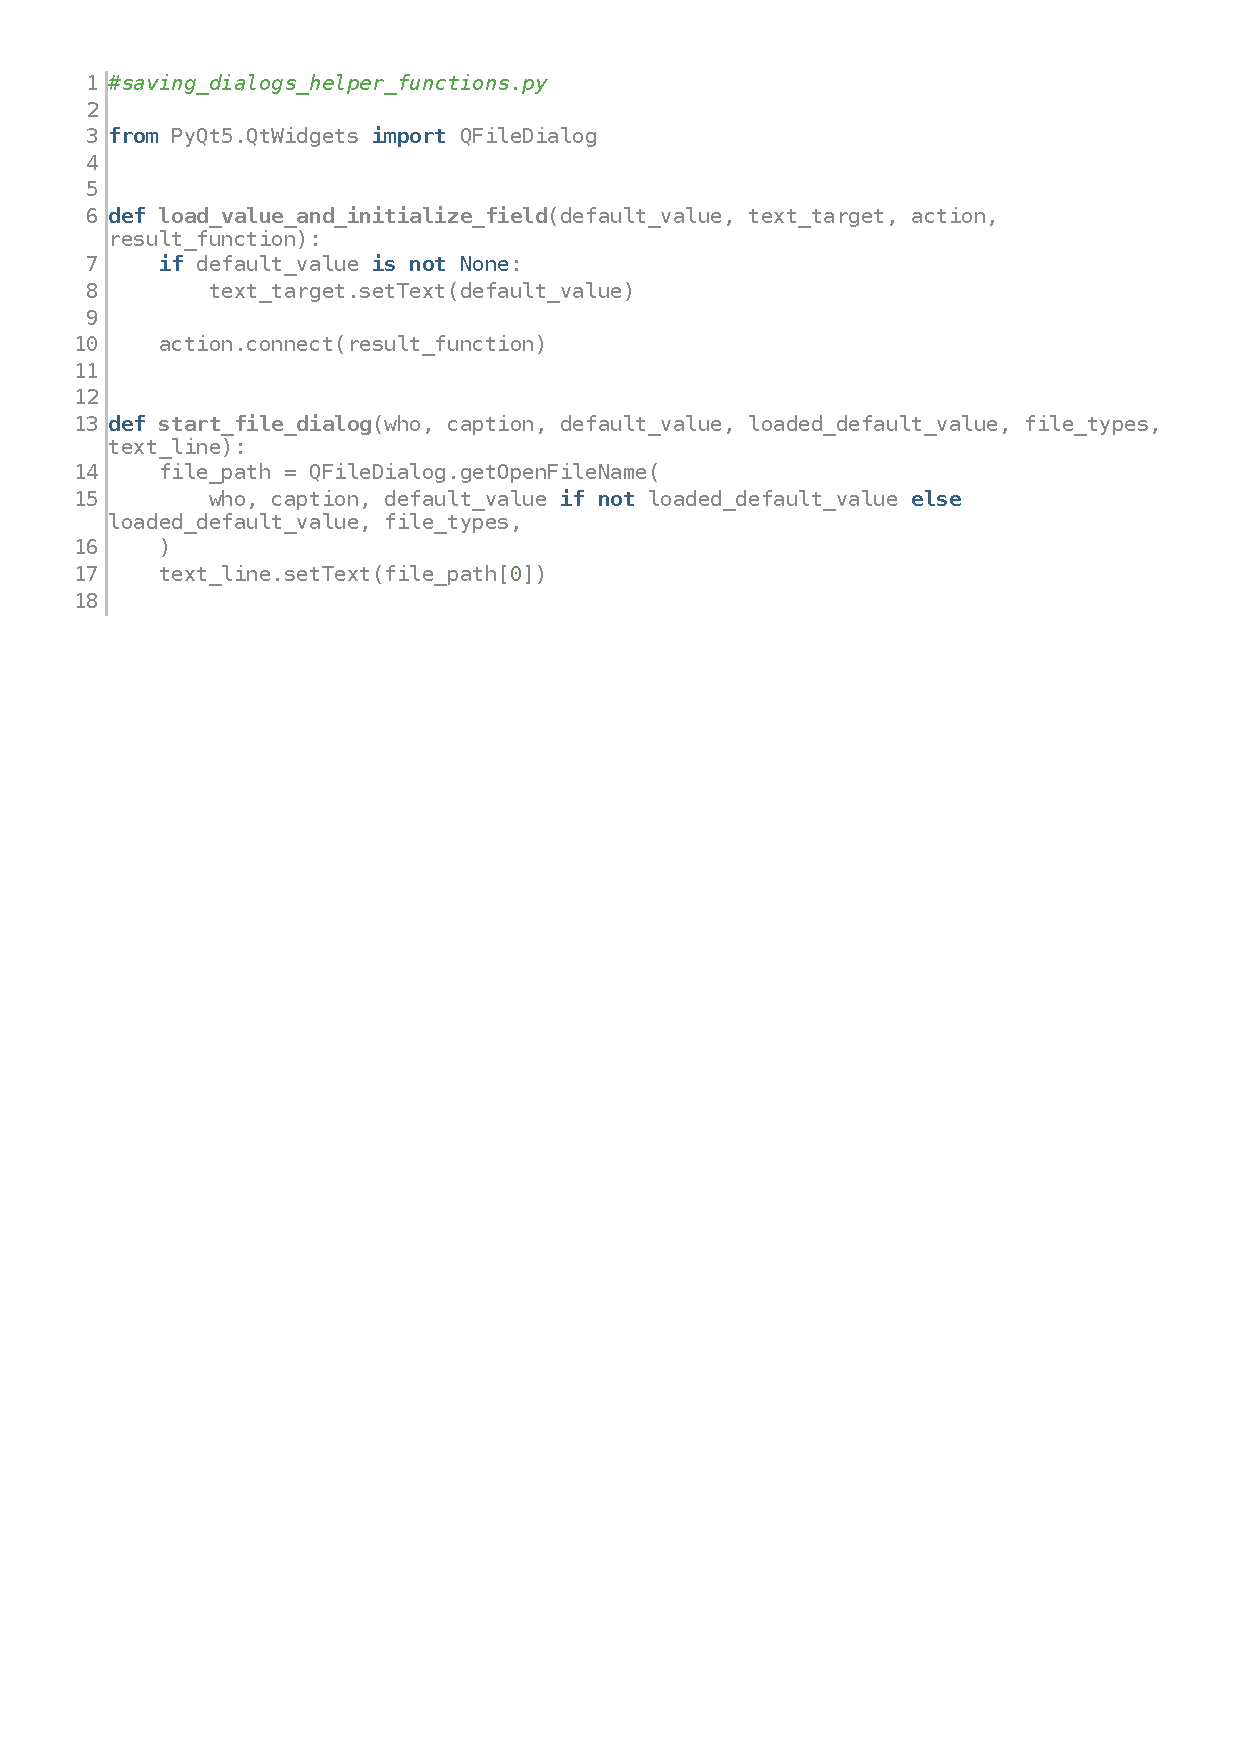
\includepdf[pages=-,pagecommand={},delta=3mm 3mm, frame = true, width=\textwidth]{saving_dialogs_helper_functions.pdf}
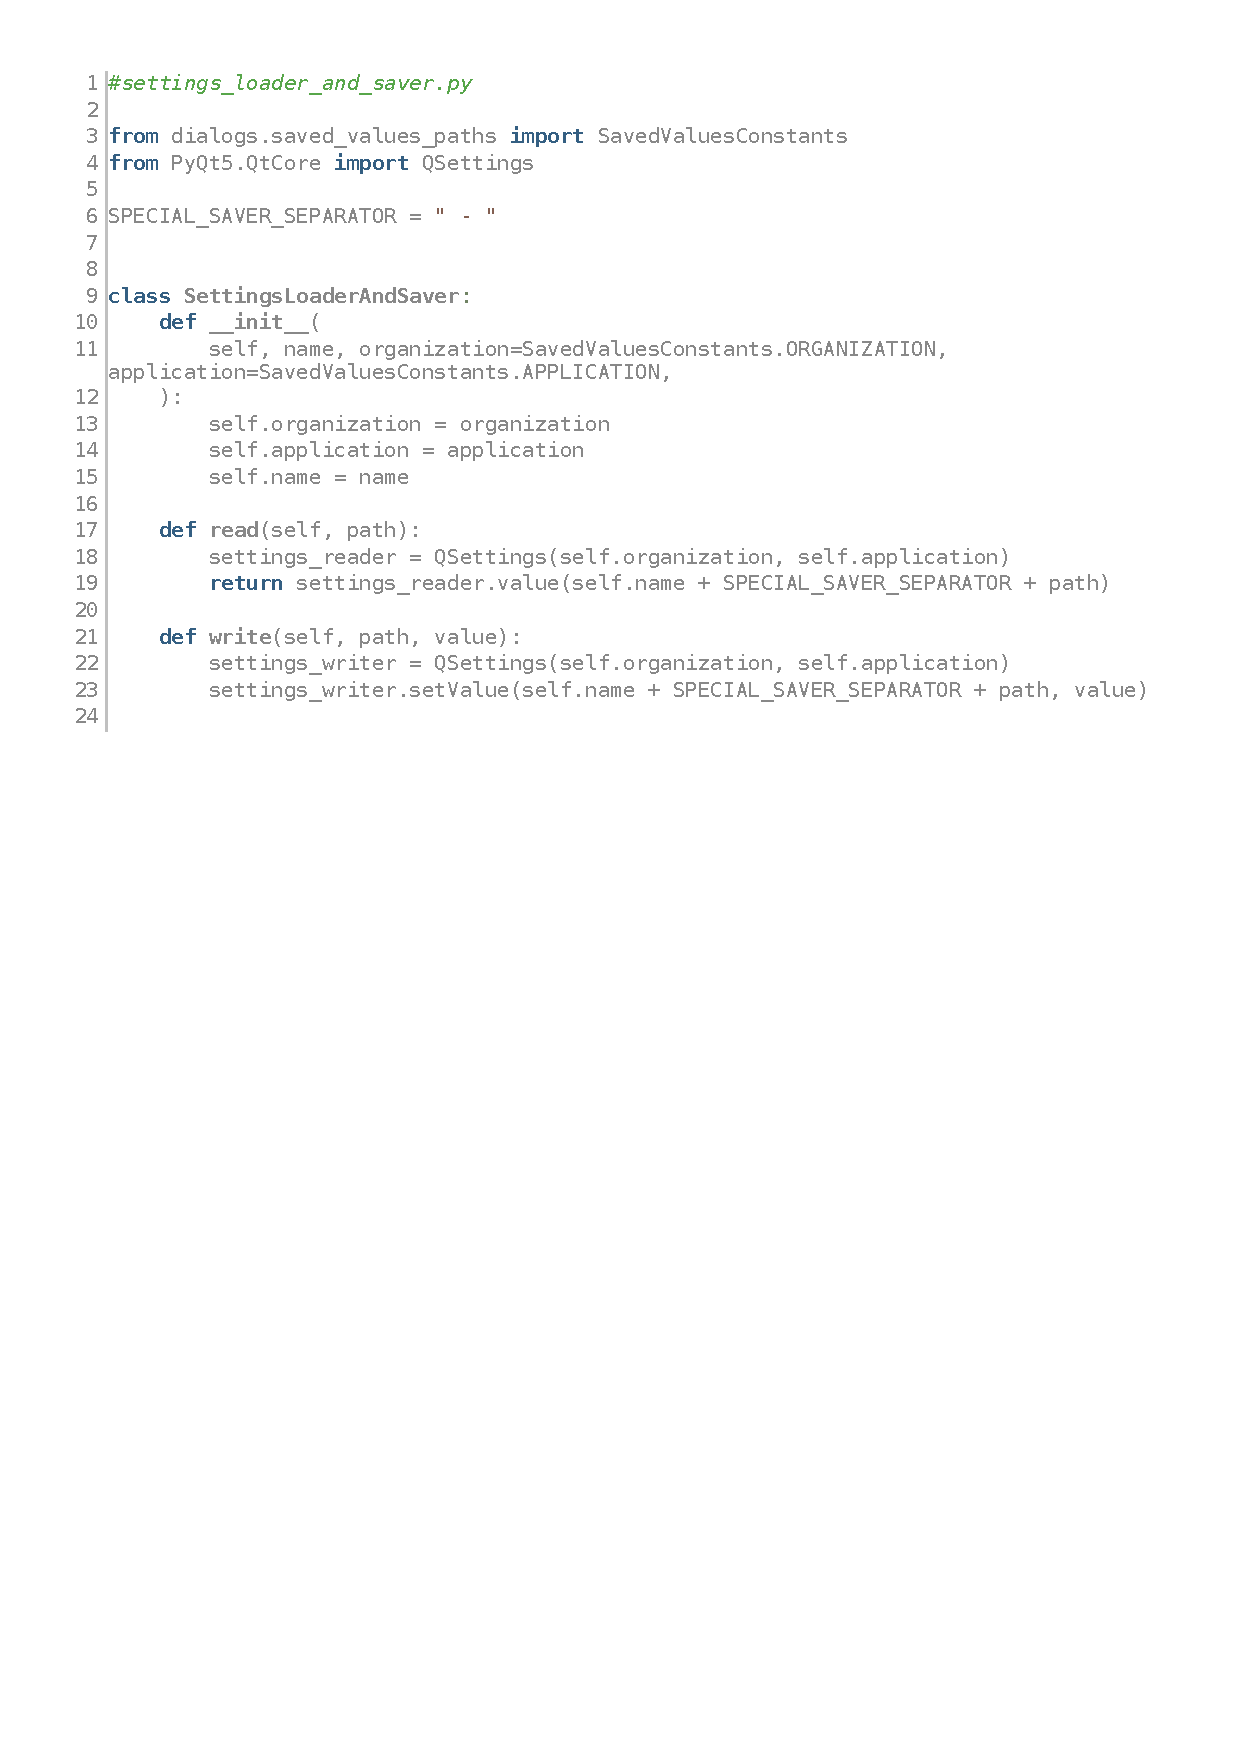
\includepdf[pages=-,pagecommand={},delta=3mm 3mm, frame = true, width=\textwidth]{settings_loader_and_saver.pdf}
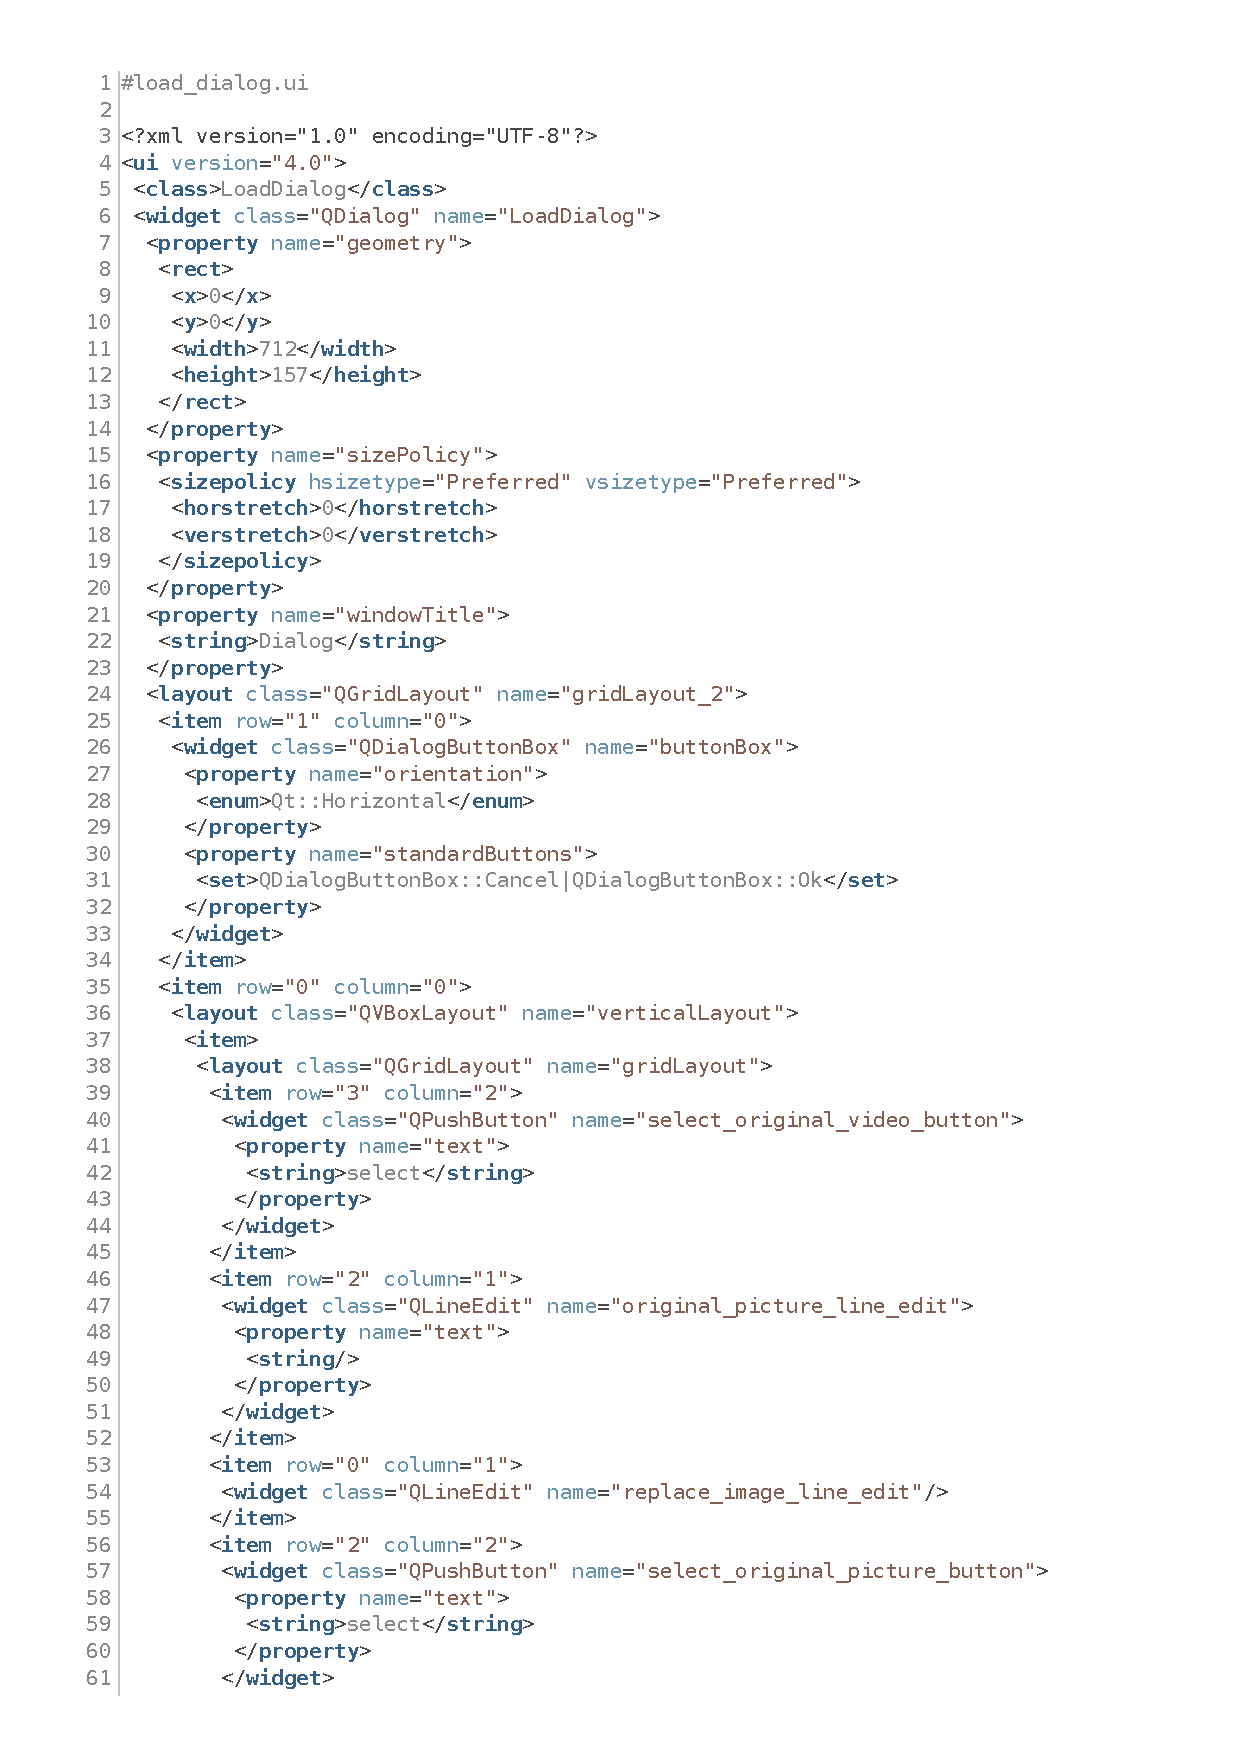
\includepdf[pages=-,pagecommand={},delta=3mm 3mm, frame = true, width=\textwidth]{load_dialog.pdf}
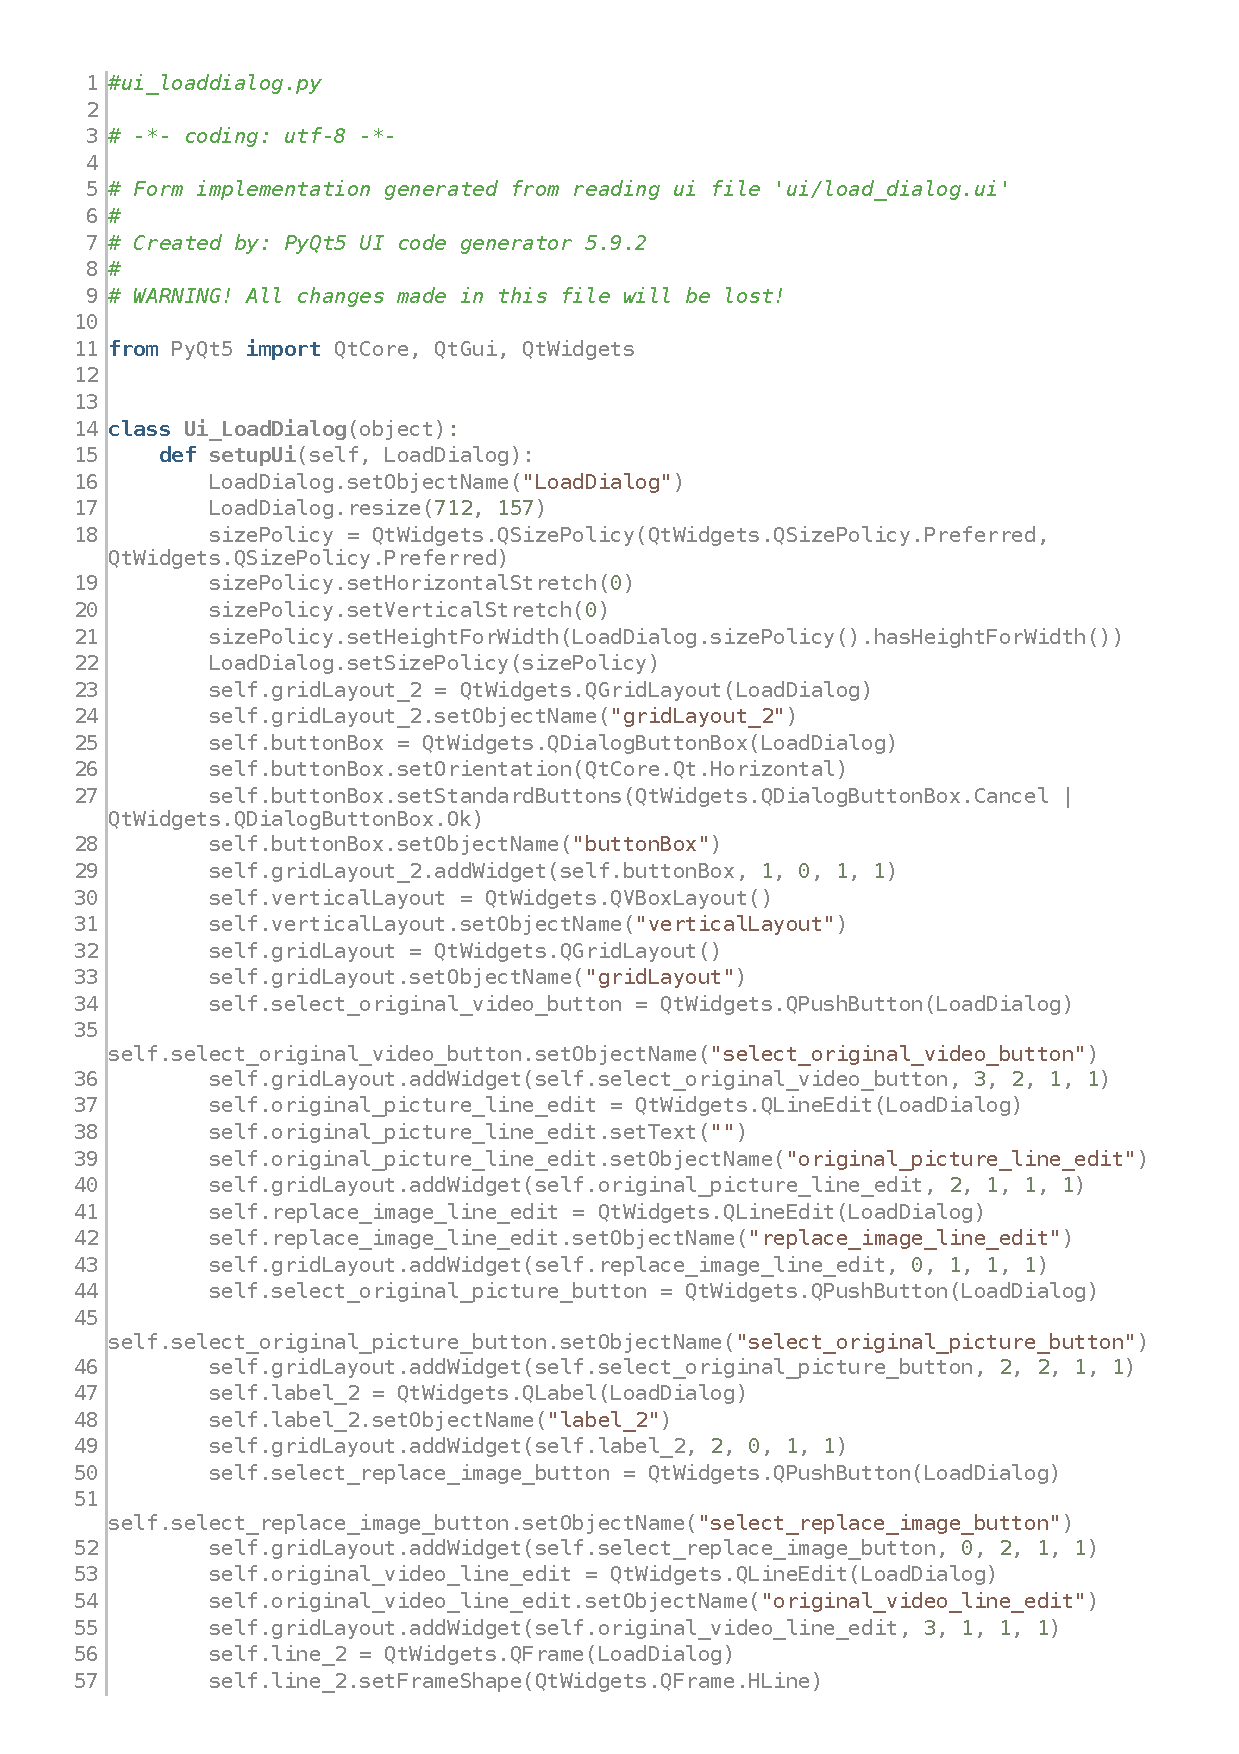
\includepdf[pages=-,pagecommand={},delta=3mm 3mm, frame = true, width=\textwidth]{ui_loaddialog.pdf}

\section{Color Picker}
\noindent A color picker has been added with the main window of GUI for user to pick the exact color of post-it note to replace in order to have more precise detection.      \\ \par

\begin{figure}[h!]
\centering
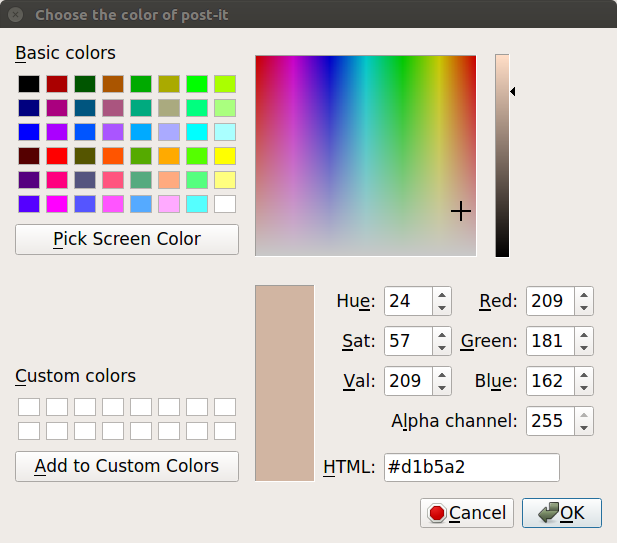
\includegraphics[width=.69\textwidth]{colorpicker.png}
\caption{A color picker for more precise detection of the color of post-it}
\end{figure}

\newpage
\section{MainWindow}
\noindent The main window of post-it replacer has three groups: replacement result groupbox, replace image groupbox and original source groupbox, which aimed at showing each part of the resources and the replacement result at the same time.      \\ \par

\begin{figure}[h!]
\centering
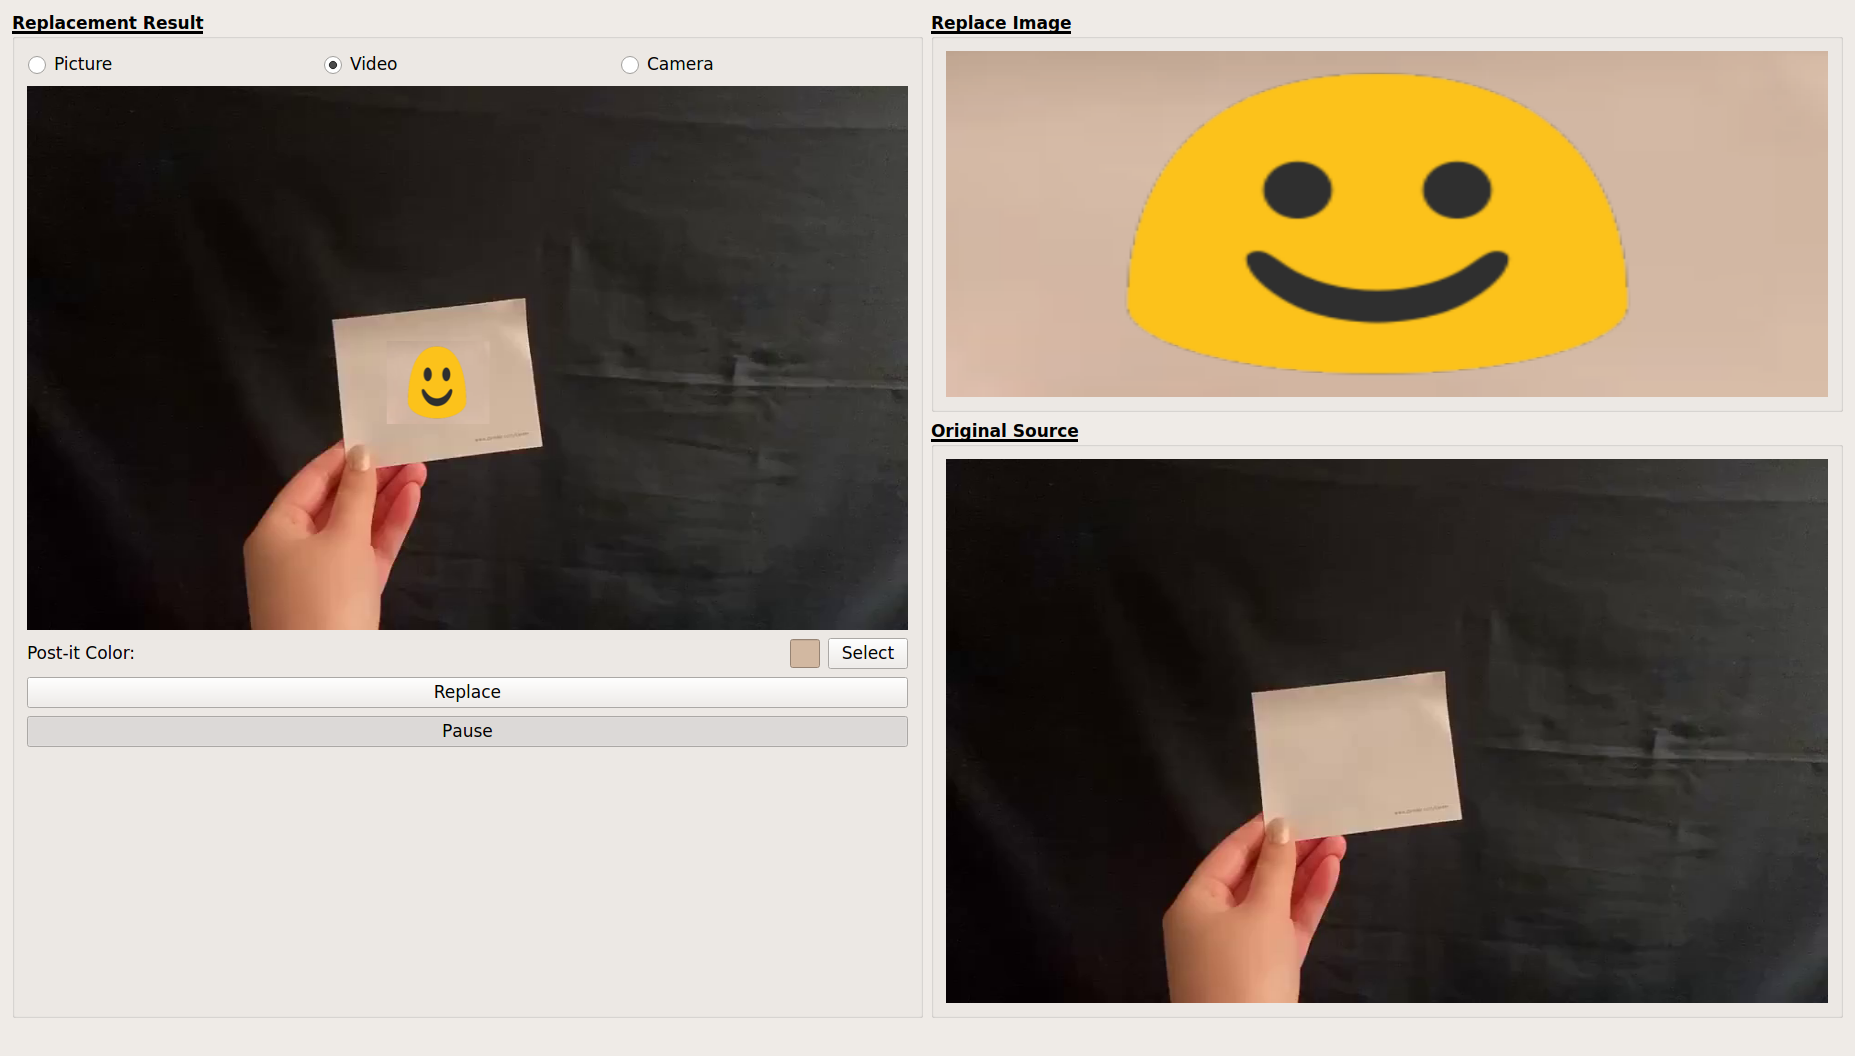
\includegraphics[width=.9\textwidth]{replace.png}
\caption{Main window showing original source, replace image and replacement result at the same time in the video mode}
\end{figure}


\newpage
\subsection{Code}
\begin{itemize}
\item mainwindow.ui
\item ui{\_}mainwindow.py
\item main{\_}window.py
\item post{\_}it{\_}replace.py
\end{itemize}

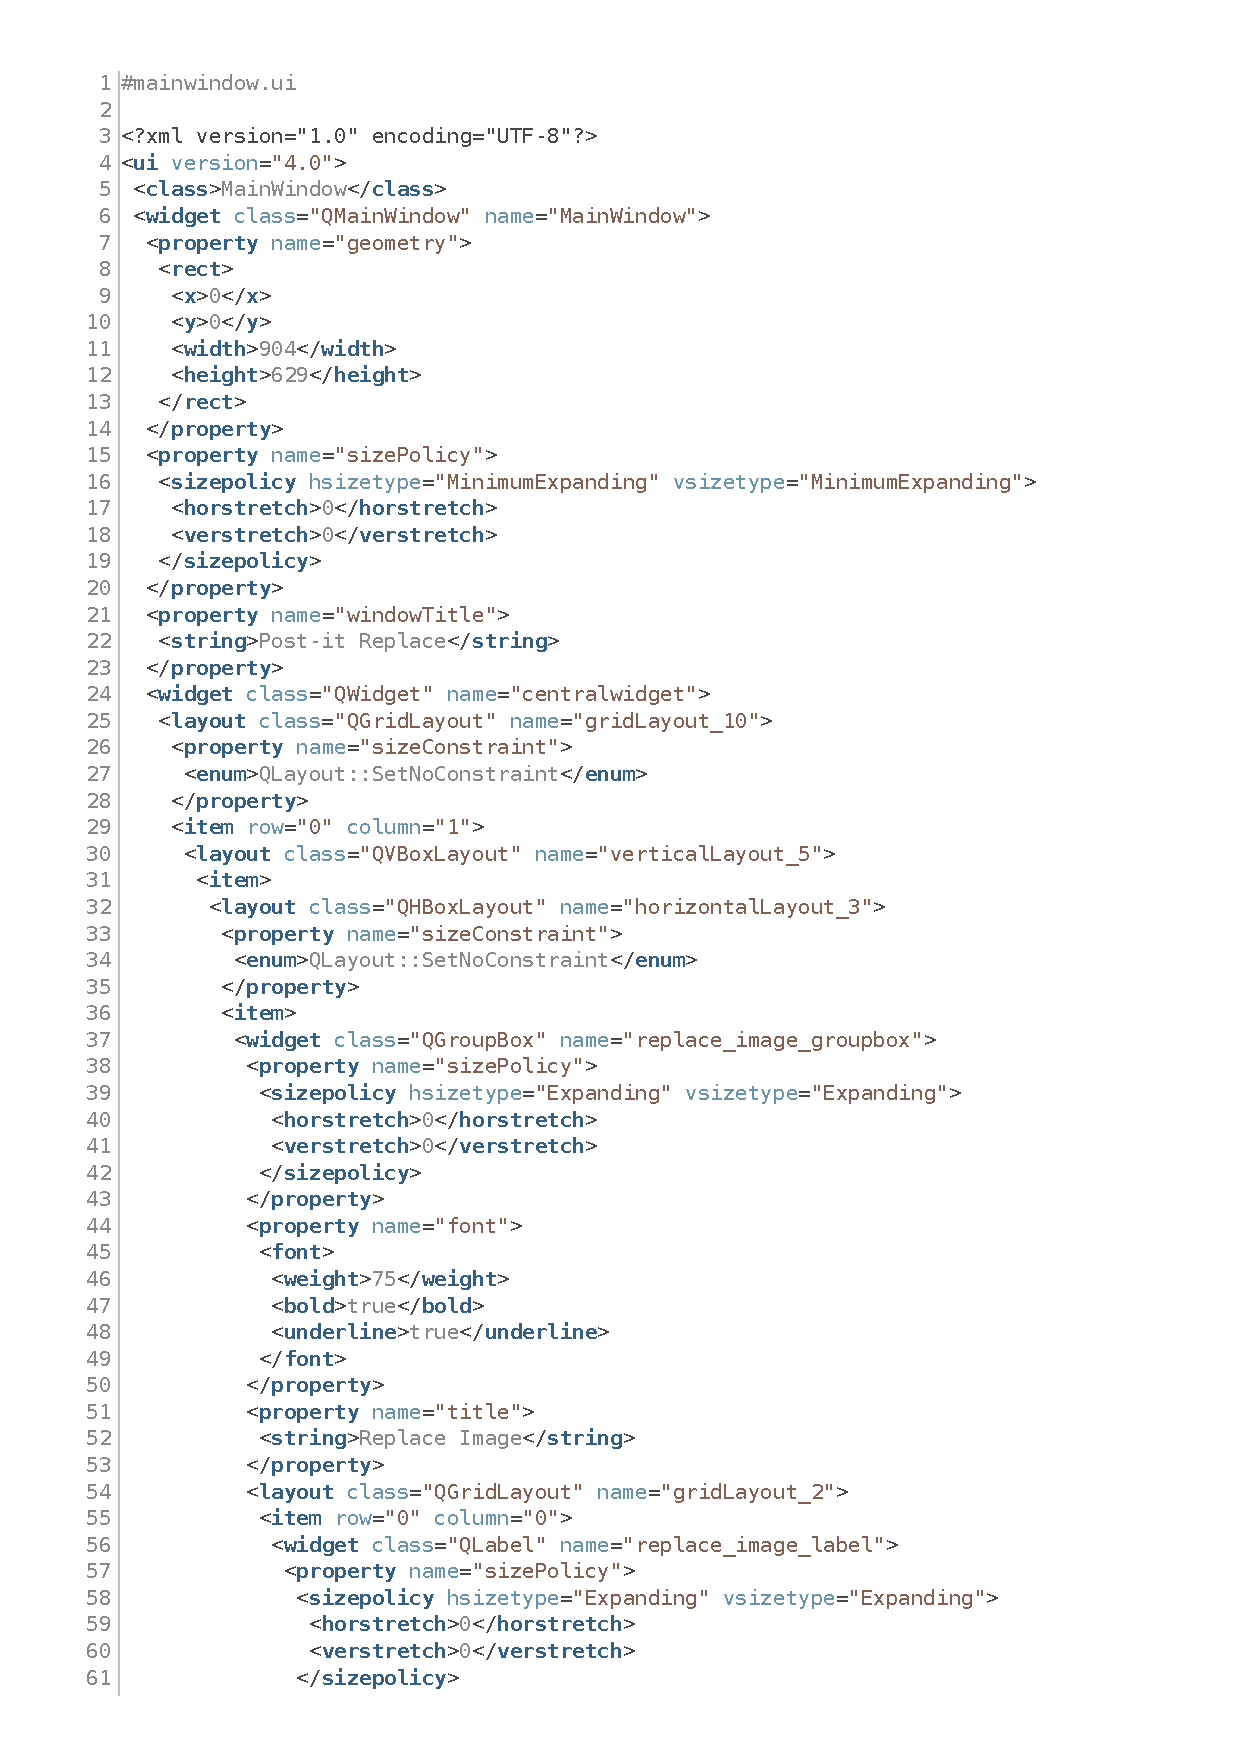
\includepdf[pages=-,pagecommand={},delta=3mm 3mm, frame = true, width=\textwidth]{mainwindow_ui.pdf}
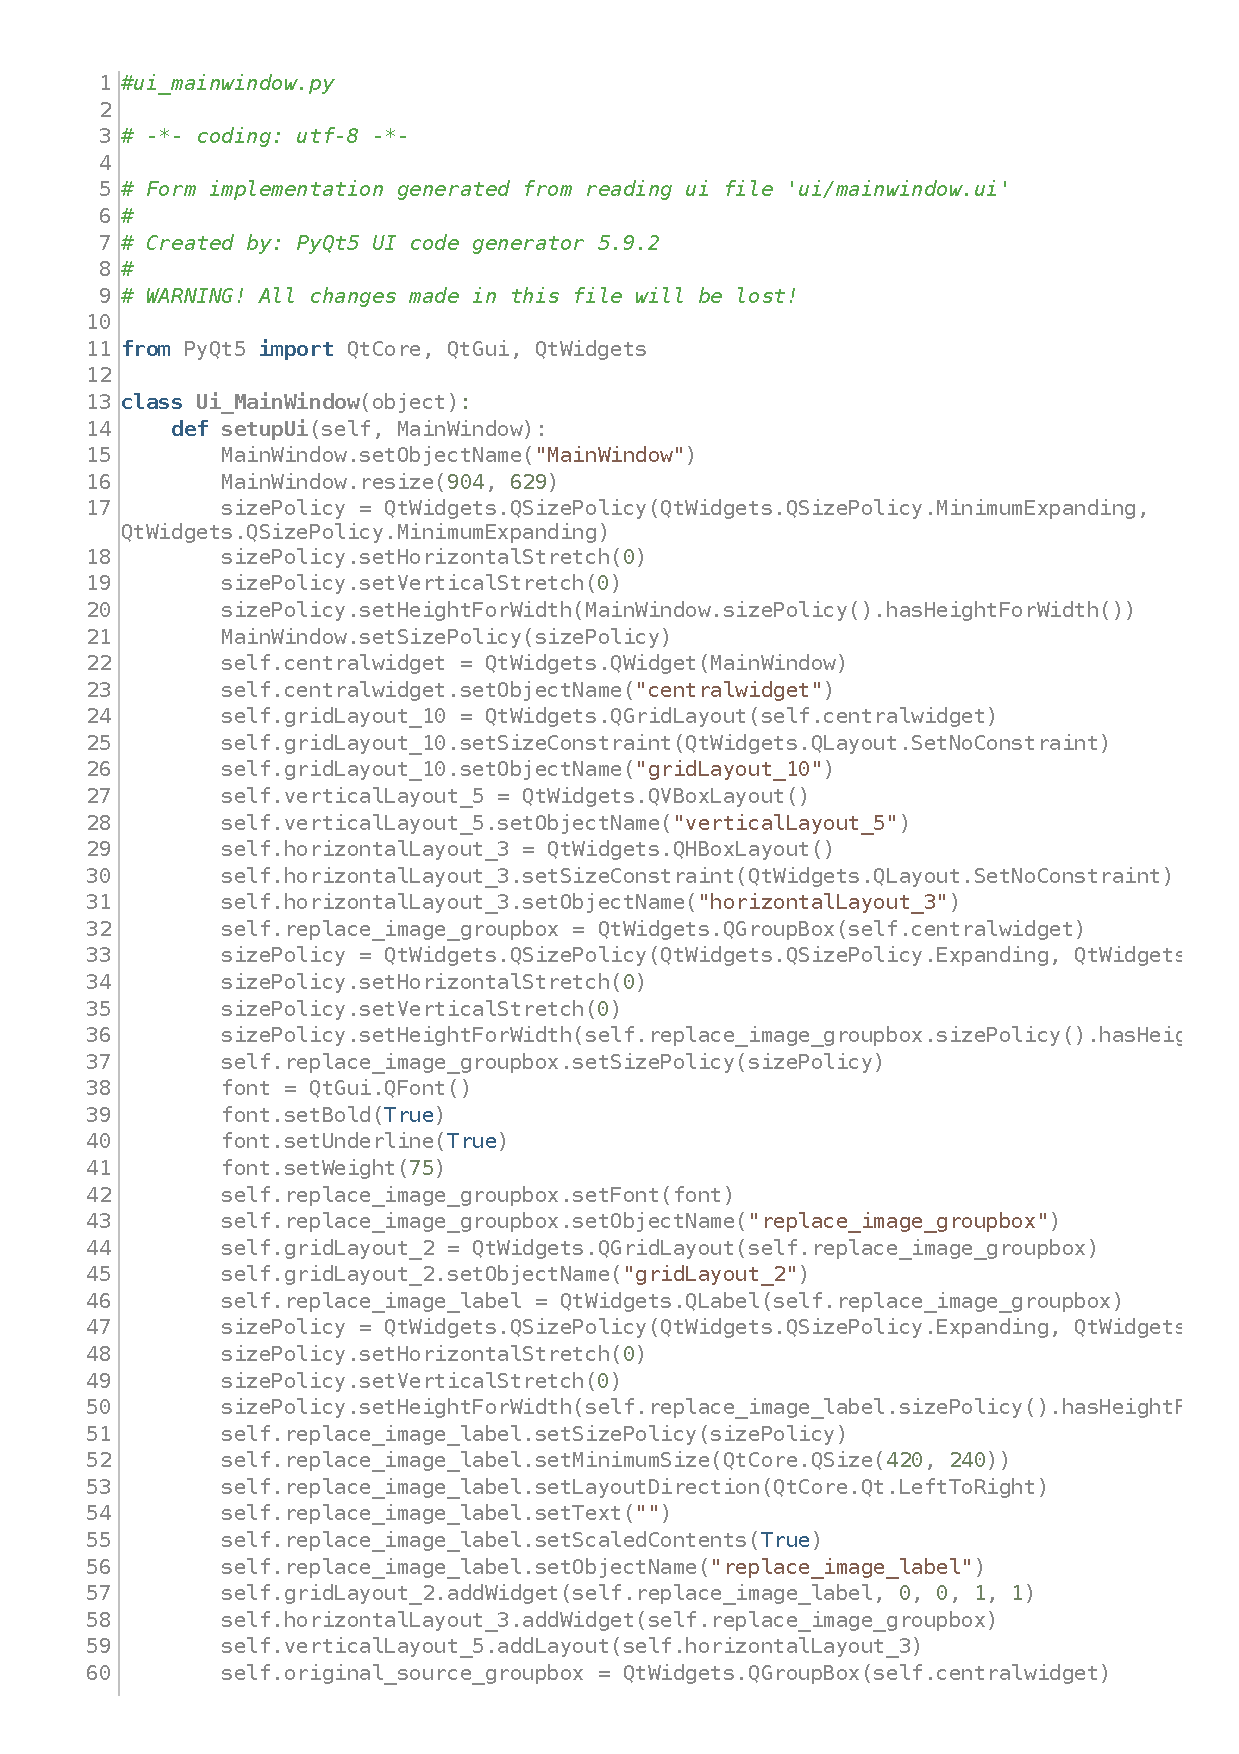
\includepdf[pages=-,pagecommand={},delta=3mm 3mm, frame = true, width=\textwidth]{mainwindow.pdf}
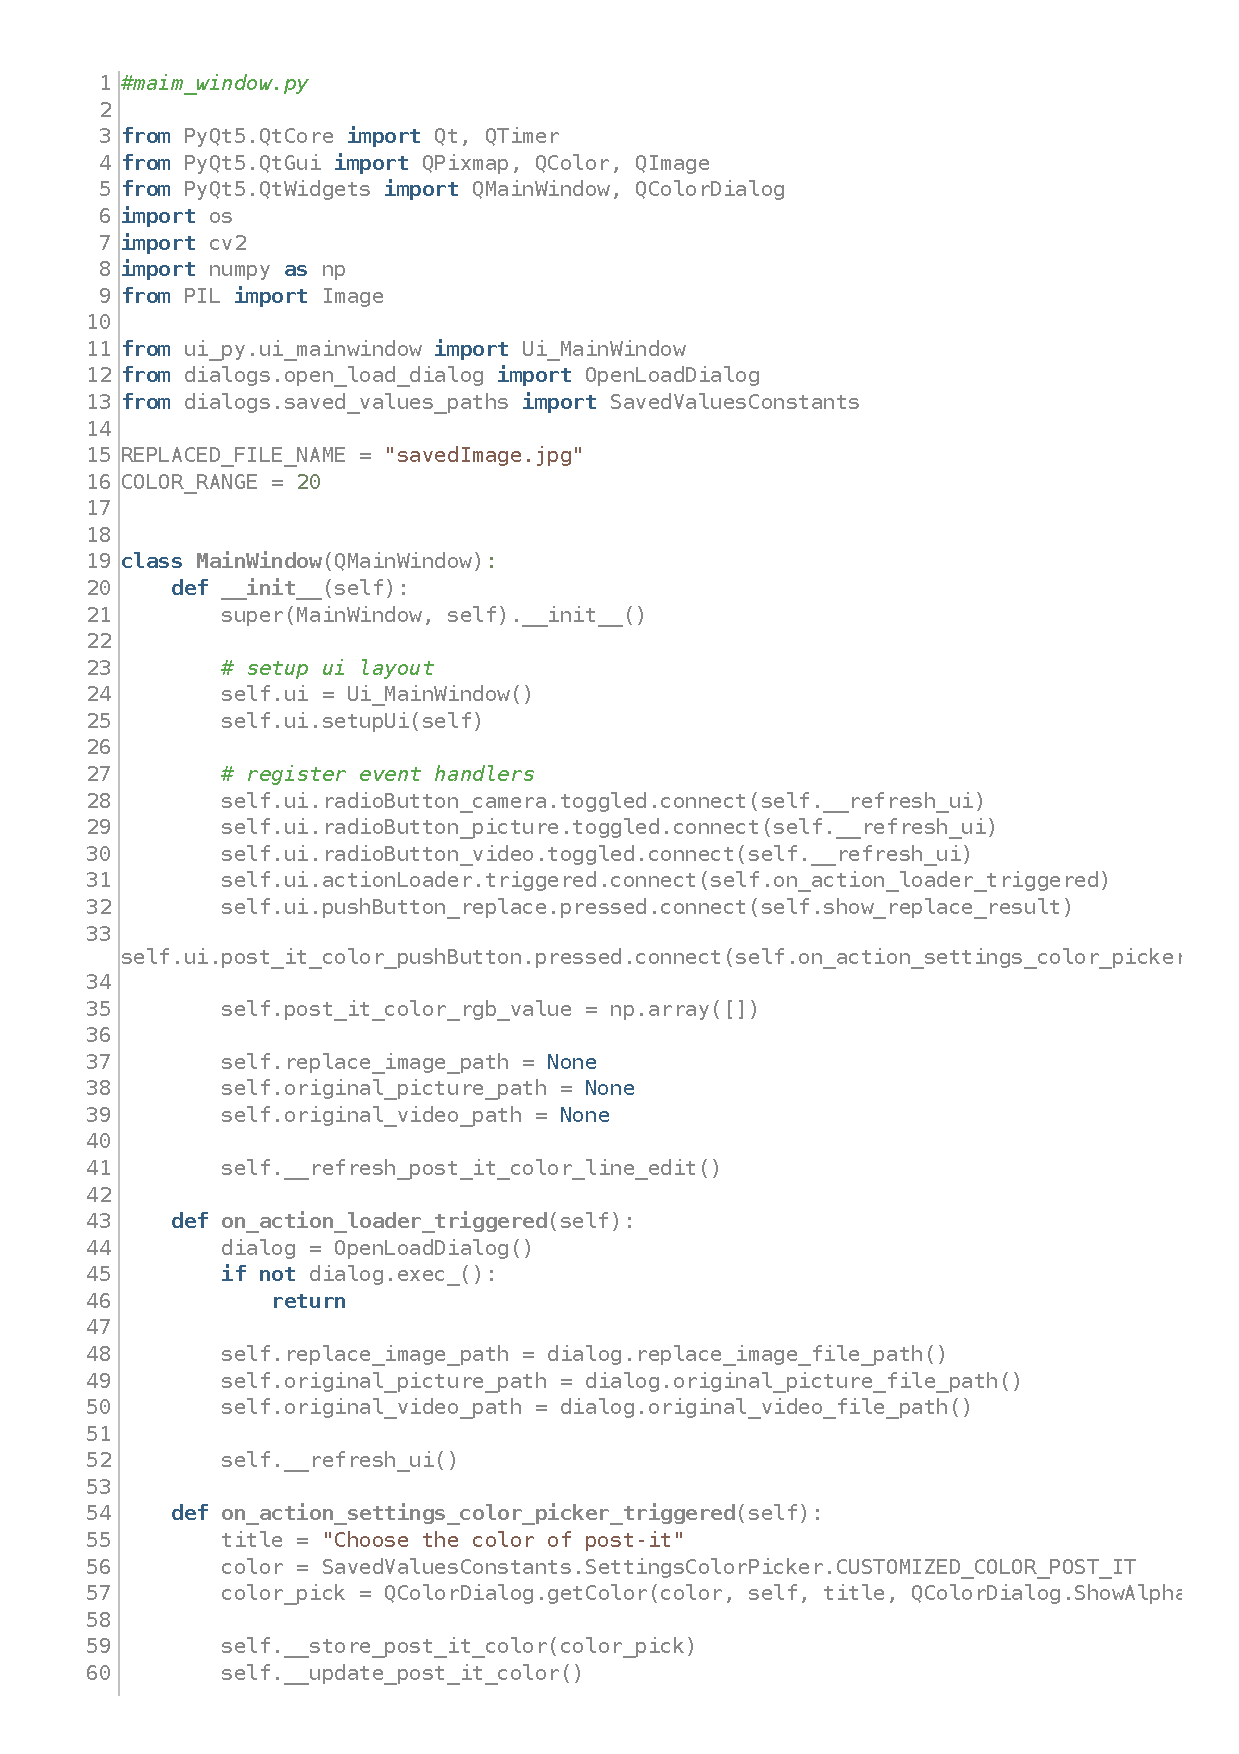
\includepdf[pages=-,pagecommand={},delta=3mm 3mm, frame = true, width=\textwidth]{main_window.pdf}
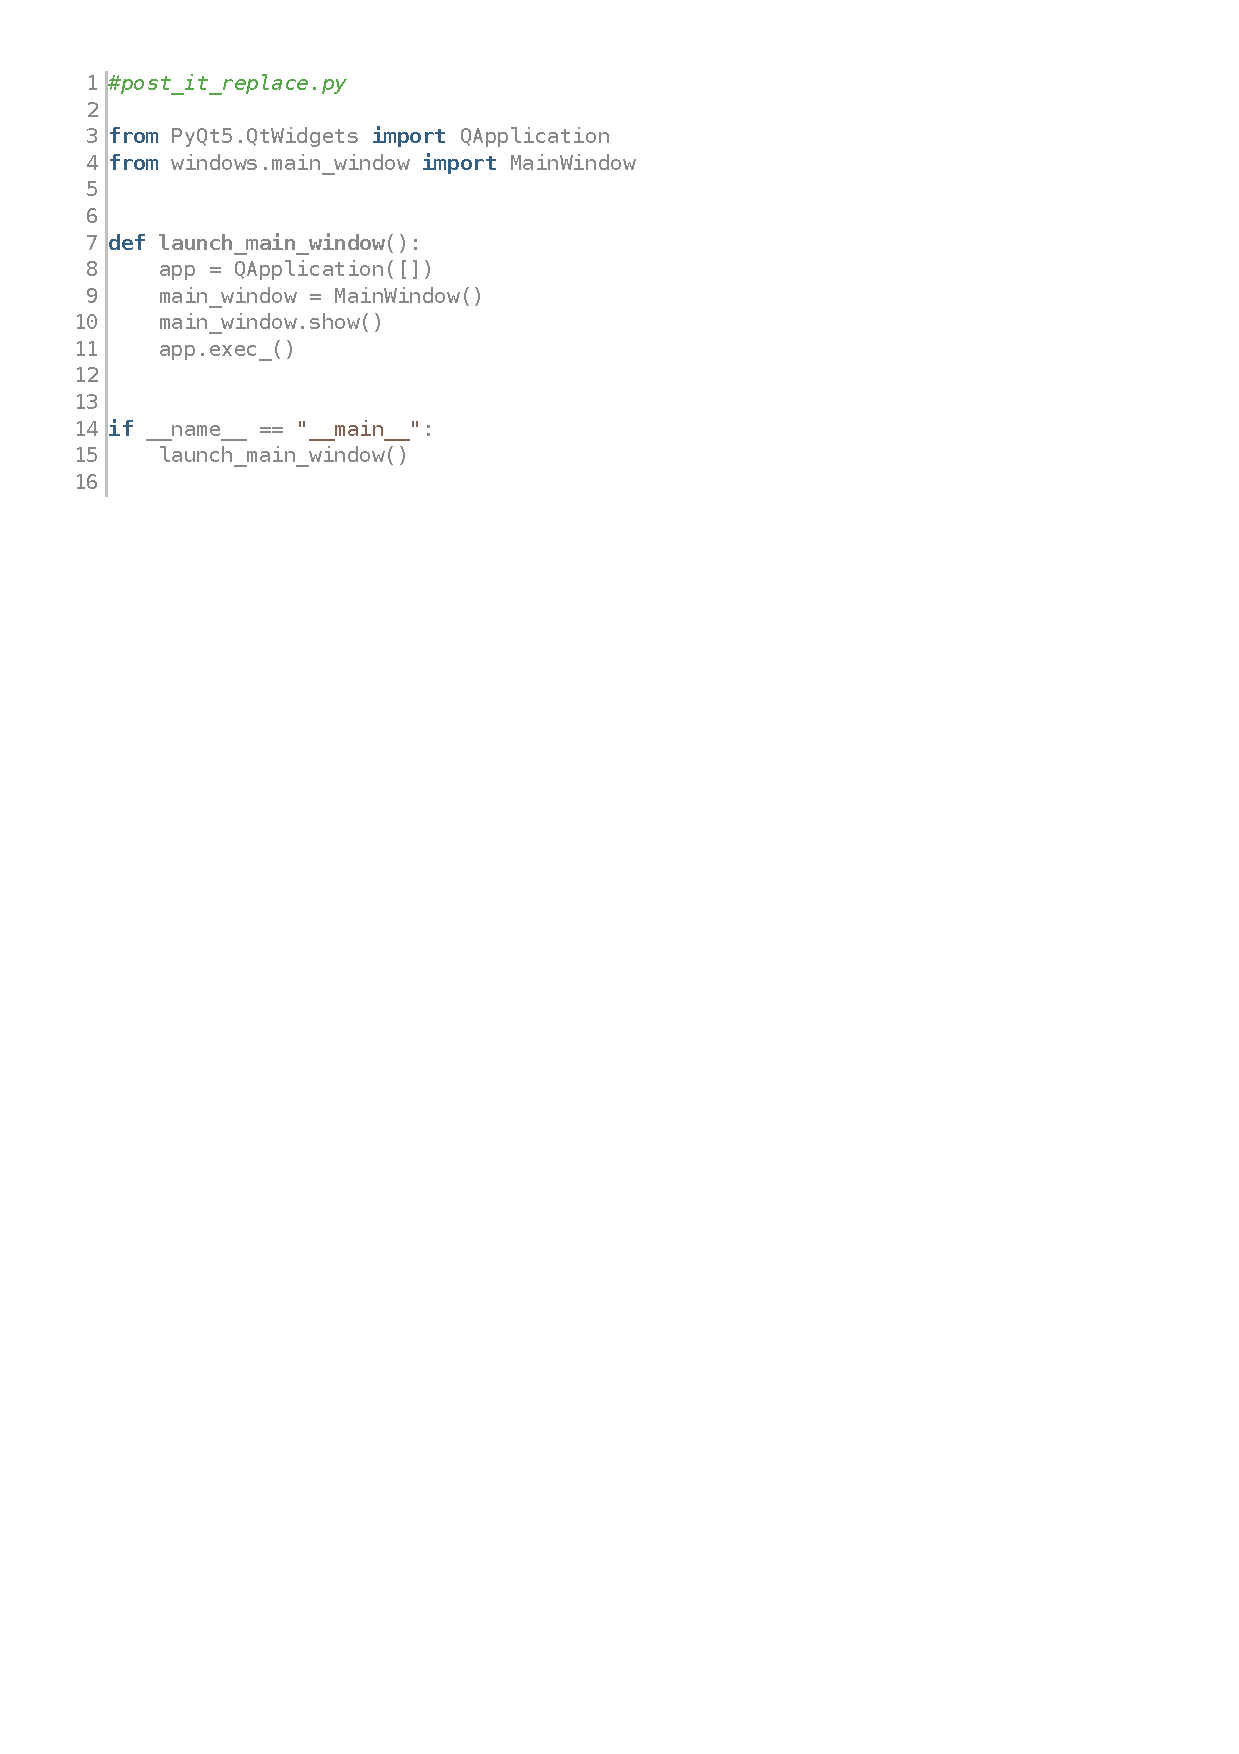
\includepdf[pages=-,pagecommand={},delta=3mm 3mm, frame = true, width=\textwidth]{post_it_replace.pdf}

\newpage
% Here is the Bibliography of this document:
\begin{thebibliography}{1}

\bibitem{GUI}
\begin{flushleft}
Wikipedia - GUI, \url{https://en.wikipedia.org/wiki/Graphical_user_interface}
\end{flushleft} 

\bibitem{Qt}
\begin{flushleft}
Wikipedia - Qt (software), \newline \url{https://en.wikipedia.org/wiki/Qt_(software)}
\end{flushleft}

\bibitem{Qt Creator}
\begin{flushleft}
Wikipedia - Qt Creator, \newline \url{https://en.wikipedia.org/wiki/Qt_Creator}
\end{flushleft}

\bibitem{pyqt5}
\begin{flushleft}
Python - Introduction to PyQt5, \newline \url{https://www.geeksforgeeks.org/python-introduction-to-pyqt5/}
\end{flushleft}

\bibitem{Visual Studio Code}
\begin{flushleft}
Wikipedia - Visual Studio Code, \newline \url{
https://en.wikipedia.org/wiki/Visual_Studio_Code}
\end{flushleft}


\bibitem{Computer Vision}
\begin{flushleft}
Wikipedia - Computer Vision, \newline \url{
https://en.wikipedia.org/wiki/Computer_vision}
\end{flushleft}


\bibitem{OpenCV-Python}
\begin{flushleft}
OpenCV-Python, \newline \url{
https://www.geeksforgeeks.org/python-opencv-cv2-imread-method/}
\end{flushleft}

\bibitem{Computer Vision for Beginners: Part 4}
\begin{flushleft}
Computer Vision for Beginners: Part 4, \newline \url{
https://towardsdatascience.com/computer-vision-for-beginners-part-4-64a8d9856208}
\end{flushleft}

\bibitem{opencv function docs}
\begin{flushleft}
opencv function docs, \newline \url{
https://docs.opencv.org/4.1.2/index.html
}
\end{flushleft}

\end{thebibliography}
\end{document}


